% Options for packages loaded elsewhere
\PassOptionsToPackage{unicode}{hyperref}
\PassOptionsToPackage{hyphens}{url}
\documentclass[
  ignorenonframetext,
]{beamer}
\newif\ifbibliography
\usepackage{pgfpages}
\setbeamertemplate{caption}[numbered]
\setbeamertemplate{caption label separator}{: }
\setbeamercolor{caption name}{fg=normal text.fg}
\beamertemplatenavigationsymbolsempty
% remove section numbering
\setbeamertemplate{part page}{
  \centering
  \begin{beamercolorbox}[sep=16pt,center]{part title}
    \usebeamerfont{part title}\insertpart\par
  \end{beamercolorbox}
}
\setbeamertemplate{section page}{
  \centering
  \begin{beamercolorbox}[sep=12pt,center]{section title}
    \usebeamerfont{section title}\insertsection\par
  \end{beamercolorbox}
}
\setbeamertemplate{subsection page}{
  \centering
  \begin{beamercolorbox}[sep=8pt,center]{subsection title}
    \usebeamerfont{subsection title}\insertsubsection\par
  \end{beamercolorbox}
}
% Prevent slide breaks in the middle of a paragraph
\widowpenalties 1 10000
\raggedbottom
\AtBeginPart{
  \frame{\partpage}
}
\AtBeginSection{
  \ifbibliography
  \else
    \frame{\sectionpage}
  \fi
}
\AtBeginSubsection{
  \frame{\subsectionpage}
}
\usepackage{iftex}
\ifPDFTeX
  \usepackage[T1]{fontenc}
  \usepackage[utf8]{inputenc}
  \usepackage{textcomp} % provide euro and other symbols
\else % if luatex or xetex
  \usepackage{unicode-math} % this also loads fontspec
  \defaultfontfeatures{Scale=MatchLowercase}
  \defaultfontfeatures[\rmfamily]{Ligatures=TeX,Scale=1}
\fi
\usepackage{lmodern}
\ifPDFTeX\else
  % xetex/luatex font selection
\fi
% Use upquote if available, for straight quotes in verbatim environments
\IfFileExists{upquote.sty}{\usepackage{upquote}}{}
\IfFileExists{microtype.sty}{% use microtype if available
  \usepackage[]{microtype}
  \UseMicrotypeSet[protrusion]{basicmath} % disable protrusion for tt fonts
}{}
\makeatletter
\@ifundefined{KOMAClassName}{% if non-KOMA class
  \IfFileExists{parskip.sty}{%
    \usepackage{parskip}
  }{% else
    \setlength{\parindent}{0pt}
    \setlength{\parskip}{6pt plus 2pt minus 1pt}}
}{% if KOMA class
  \KOMAoptions{parskip=half}}
\makeatother
\usepackage{longtable,booktabs,array}
\newcounter{none} % for unnumbered tables
\usepackage{calc} % for calculating minipage widths
\usepackage{caption}
% Make caption package work with longtable
\makeatletter
\def\fnum@table{\tablename~\thetable}
\makeatother
\usepackage{graphicx}
\makeatletter
\newsavebox\pandoc@box
\newcommand*\pandocbounded[1]{% scales image to fit in text height/width
  \sbox\pandoc@box{#1}%
  \Gscale@div\@tempa{\textheight}{\dimexpr\ht\pandoc@box+\dp\pandoc@box\relax}%
  \Gscale@div\@tempb{\linewidth}{\wd\pandoc@box}%
  \ifdim\@tempb\p@<\@tempa\p@\let\@tempa\@tempb\fi% select the smaller of both
  \ifdim\@tempa\p@<\p@\scalebox{\@tempa}{\usebox\pandoc@box}%
  \else\usebox{\pandoc@box}%
  \fi%
}
% Set default figure placement to htbp
\def\fps@figure{htbp}
\makeatother
\setlength{\emergencystretch}{3em} % prevent overfull lines
\providecommand{\tightlist}{%
  \setlength{\itemsep}{0pt}\setlength{\parskip}{0pt}}
% Auto-generated by infrastructure/rendering/_pdf_latex_helpers.py::extract_math_font_preamble.
% Minimal header passed to Pandoc via -H so Beamer slides pick up the same math font
% as the combined-PDF path. Adjust the manuscript's preamble.md to change the font globally.
\usepackage{unicode-math}
\setmathfont{latinmodern-math.otf}

% Slide layout defaults for warning-clean scientific decks.
\usepackage{etoolbox}
\IfFileExists{xurl.sty}{\usepackage{xurl}}{}
\IfFileExists{seqsplit.sty}{\usepackage{seqsplit}}{\newcommand{\seqsplit}[1]{#1}}
\protected\def\breakseq#1{\seqsplit{#1}}
\protected\def\breaktt#1{\begingroup\ttfamily\seqsplit{#1}\endgroup}
\setlength{\emergencystretch}{6em}
\tolerance=5000
\hbadness=10000
\hfuzz=1pt
\setlength{\tabcolsep}{2pt}
\AtBeginEnvironment{longtable}{\tiny\renewcommand{\arraystretch}{0.86}\setlength{\tabcolsep}{1pt}}
\AtBeginEnvironment{tabular}{\tiny\renewcommand{\arraystretch}{0.86}\setlength{\tabcolsep}{1pt}}

% Natbib and cross-reference fallbacks — slides don't load natbib
% or cleveref, but combined-PDF manuscript prose may emit these
% commands. The fallback renders citations as a bracketed key list
% and cross-references as detokenized labels so slides don't fail on
% undefined control sequences or raw underscores. \providecommand is
% a no-op if packages load later.
\providecommand{\citep}[1]{[#1]}
\providecommand{\citet}[1]{#1}
\providecommand{\citealp}[1]{#1}
\providecommand{\citeauthor}[1]{#1}
\providecommand{\citeyear}[1]{#1}
\providecommand{\cref}[1]{\texttt{\detokenize{#1}}}
\providecommand{\Cref}[1]{\texttt{\detokenize{#1}}}
\usepackage{bookmark}
\IfFileExists{xurl.sty}{\usepackage{xurl}}{} % add URL line breaks if available
\urlstyle{same}
% fallback for those not using the hyperref driver hyperxmp:
\makeatletter
\@ifundefined{xmpquote}{\newcommand{\xmpquote}[1]{#1}}{}
\makeatother
\hypersetup{
  hidelinks,
  pdfcreator={LaTeX via pandoc}}

\author{\texorpdfstring{}{}}
\date{}

\begin{document}

\section{Results: Provenance, Density, and Resolved Manuscript
Surface}\label{results-provenance-density-and-resolved-manuscript-surface}

\begin{frame}[allowframebreaks]{Results: Provenance, Density, and
Resolved Manuscript Surface}
The generated plan enables 11 of 11 manuscript sections and fills 40
token choice(s). Category density is adjectives: 2, artifacts: 8,
audiences: 4, constraints: 3, failures: 3, measures: 6, methods: 1,
nouns: 5, qualities: 3, verbs: 5. The result figures are generated from
the same token plan that writes the inventory table, so visual and
tabular claims share one source.

The configured results moves are report token density, show resolved
section coverage, bind every manuscript token to provenance, and connect
the figure and inventory to the same plan. The important result is
therefore not a surprising word choice; it is the survival of
traceability through a complete render path. Each token row records the
variable, category, selected value, section, and config pointer that
produced it.

The resolved manuscript also demonstrates the intended failure boundary.
If a manuscript placeholder is added without a corresponding variable,
the project test suite detects it. If a figure is referenced without
registry support, the output validator reports it. If a generated number
lacks evidence support, the evidence registry gate reports it before the
copied output stage packages deliverables.

Visualization is enabled for configured\_field\_matrix,
section\_configuration\_heatmap, field\_origin\_summary,
token\_injection\_flow, section\_token\_allocation,
provenance\_trace\_map, quality\_gate\_matrix. The configured-field
figures are generated from the same explicit/default path inventory
written to JSON; the pipeline, allocation, provenance, and gate figures
are generated from the same token plan and QA schema.

\begin{figure}
\centering
\pandocbounded{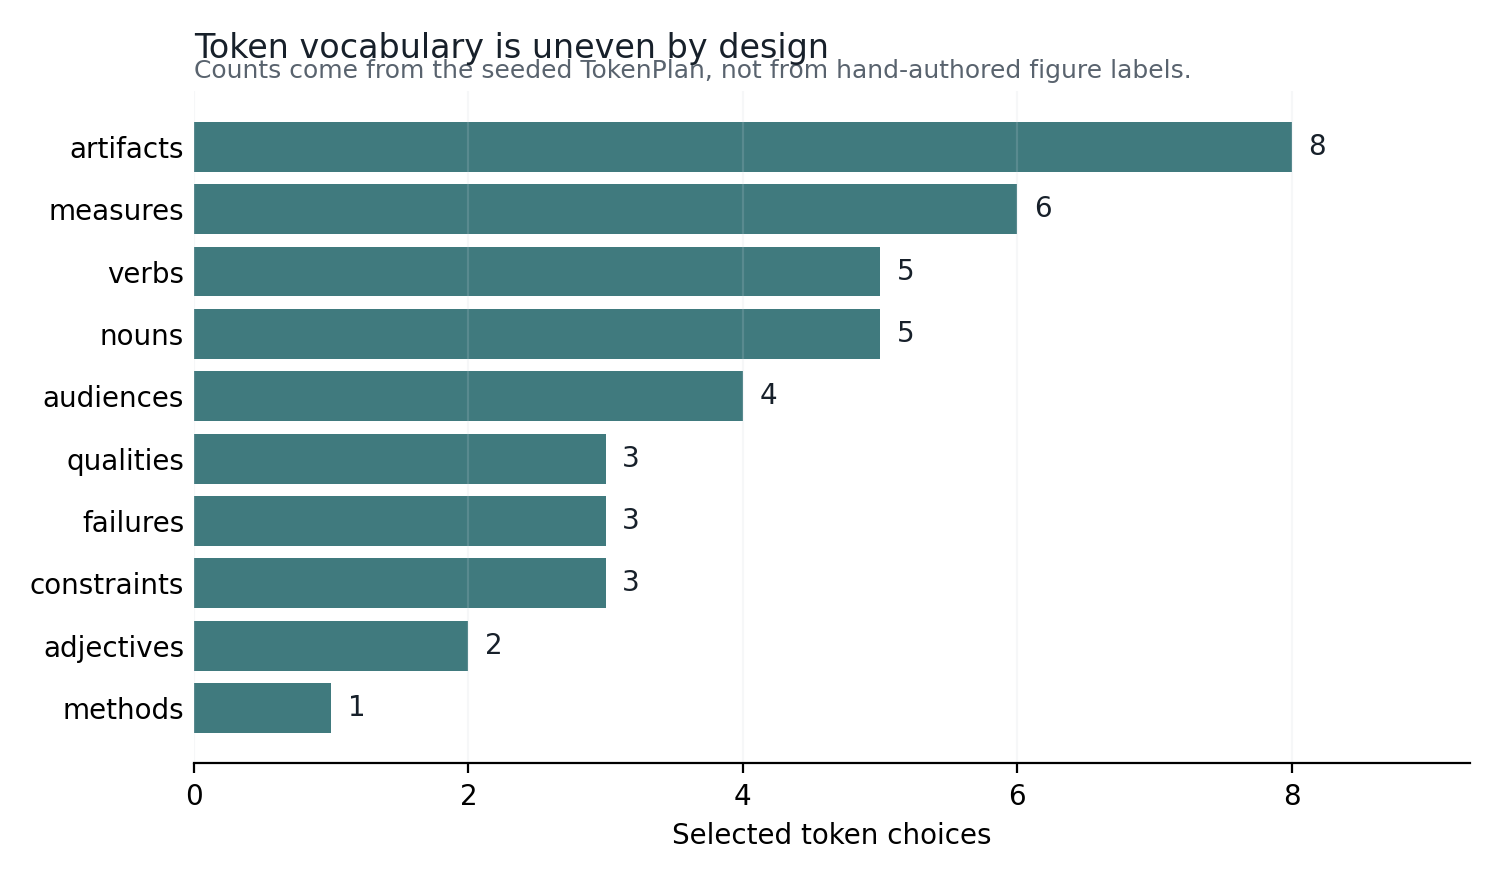
\includegraphics[keepaspectratio,alt={Token category density}]{../figures/token_density.png}}
\caption{Token category density}\label{fig:token-density}
\end{figure}

\begin{figure}
\centering
\pandocbounded{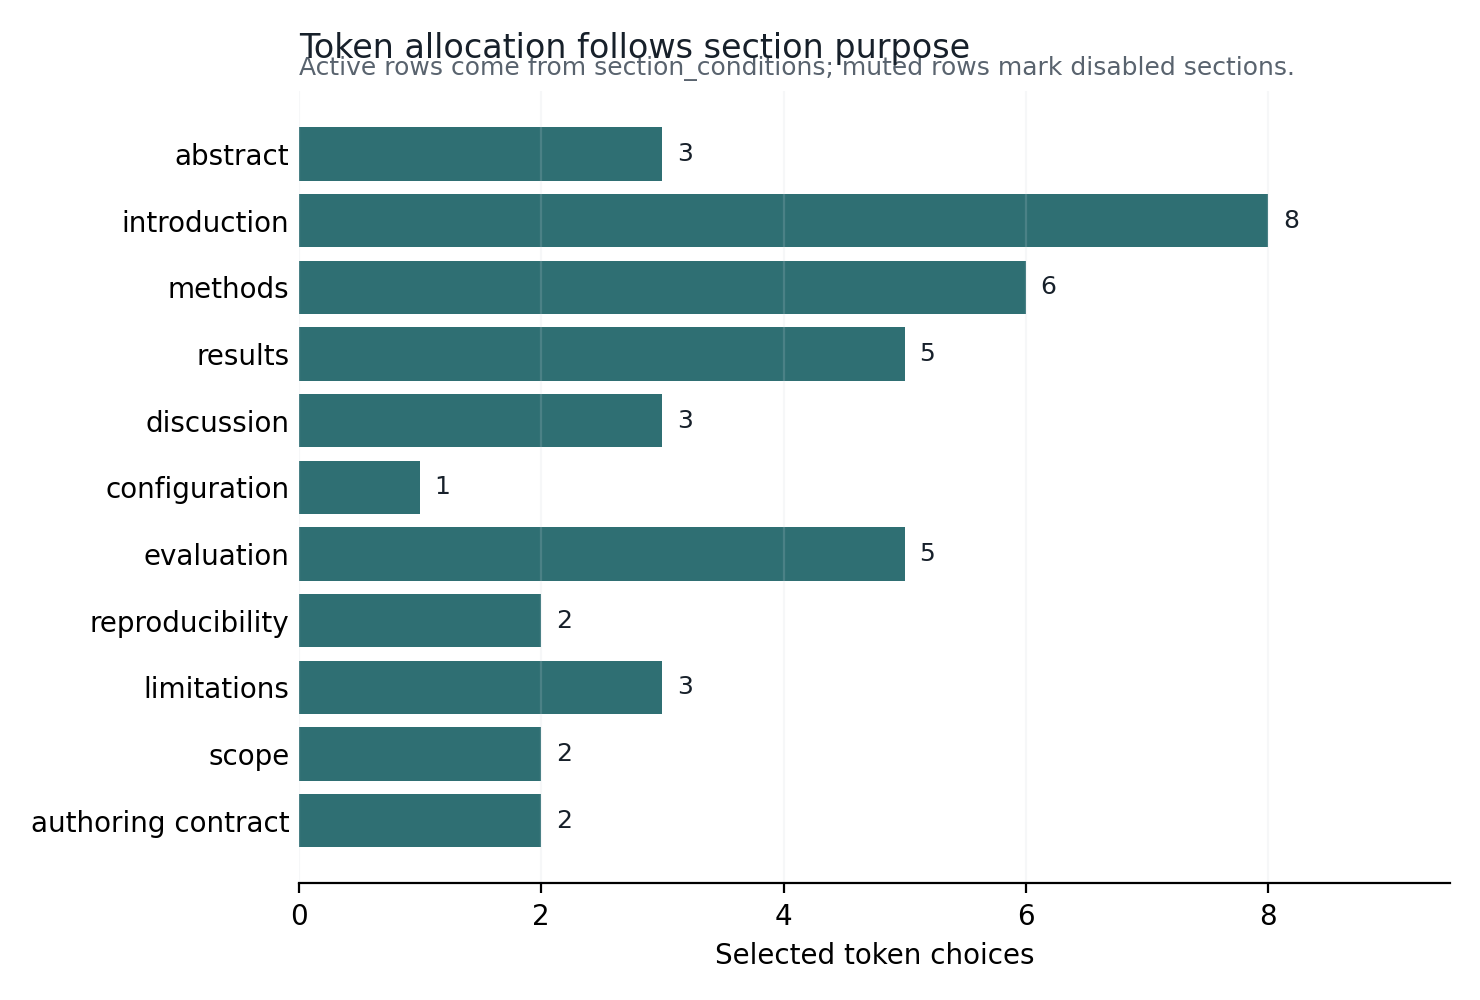
\includegraphics[keepaspectratio,alt={Section token allocation}]{../figures/section_token_allocation.png}}
\caption{Section token allocation}\label{fig:section-token-allocation}
\end{figure}

\begin{figure}
\centering
\pandocbounded{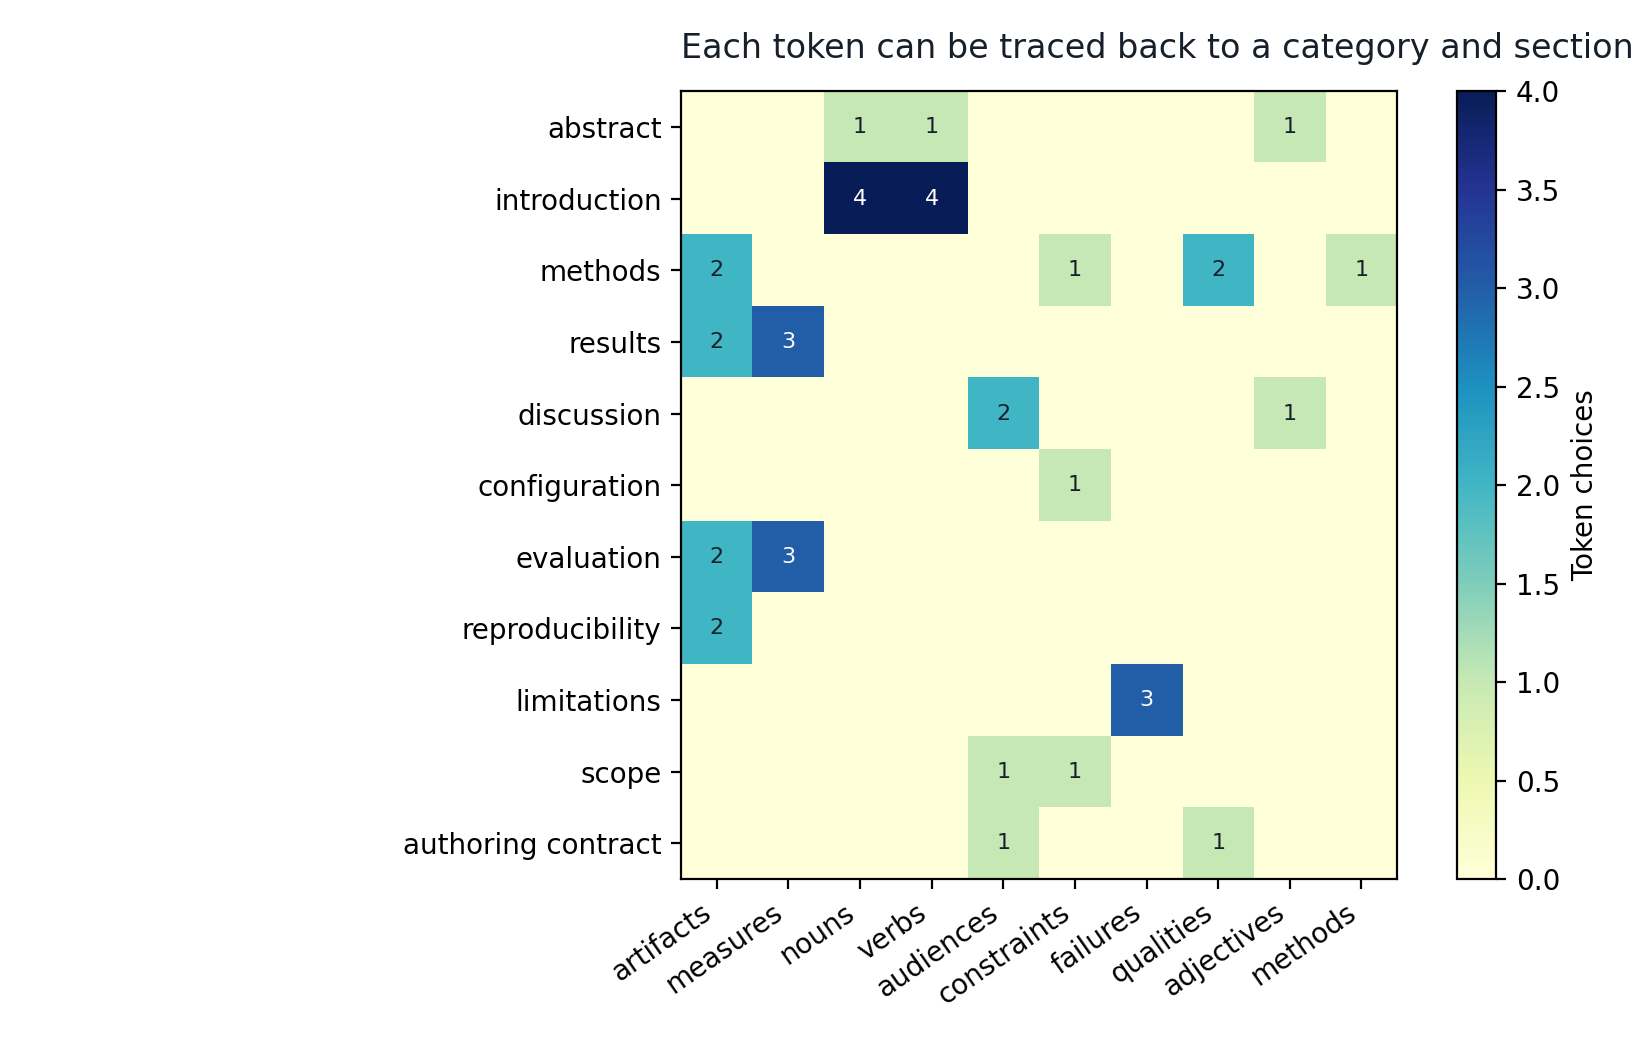
\includegraphics[keepaspectratio,alt={Provenance trace map}]{../figures/provenance_trace_map.png}}
\caption{Provenance trace map}\label{fig:provenance-trace-map}
\end{figure}
\end{frame}

\begin{frame}[fragile,allowframebreaks]{Token Inventory}
\protect\phantomsection\label{token-inventory}
{\def\LTcaptype{none} % do not increment counter
\begin{longtable}[]{@{}
  >{\raggedright\arraybackslash}p{(\linewidth - 8\tabcolsep) * \real{0.2000}}
  >{\raggedright\arraybackslash}p{(\linewidth - 8\tabcolsep) * \real{0.2000}}
  >{\raggedright\arraybackslash}p{(\linewidth - 8\tabcolsep) * \real{0.2000}}
  >{\raggedright\arraybackslash}p{(\linewidth - 8\tabcolsep) * \real{0.2000}}
  >{\raggedright\arraybackslash}p{(\linewidth - 8\tabcolsep) * \real{0.2000}}@{}}
\toprule\noalign{}
\begin{minipage}[b]{\linewidth}\raggedright
Variable
\end{minipage} & \begin{minipage}[b]{\linewidth}\raggedright
Category
\end{minipage} & \begin{minipage}[b]{\linewidth}\raggedright
Value
\end{minipage} & \begin{minipage}[b]{\linewidth}\raggedright
Section
\end{minipage} & \begin{minipage}[b]{\linewidth}\raggedright
Source
\end{minipage} \\
\midrule\noalign{}
\endhead
\texttt{STUDY\_ADJECTIVE} & adjectives & reviewable & abstract &
\texttt{manuscript/config.yaml\#madlib.lexicon.adjectives{[}5{]}} \\
\texttt{STUDY\_NOUN} & nouns & pipeline & abstract &
\texttt{manuscript/config.yaml\#madlib.lexicon.nouns{[}4{]}} \\
\texttt{STUDY\_VERB} & verbs & hydrate & abstract &
\texttt{manuscript/config.yaml\#madlib.lexicon.verbs{[}1{]}} \\
\texttt{INTRO\_NOUNS\_1} & nouns & protocol & introduction &
\texttt{manuscript/config.yaml\#madlib.lexicon.nouns{[}5{]}} \\
\texttt{INTRO\_NOUNS\_2} & nouns & section & introduction &
\texttt{manuscript/config.yaml\#madlib.lexicon.nouns{[}3{]}} \\
\texttt{INTRO\_NOUNS\_3} & nouns & lexicon & introduction &
\texttt{manuscript/config.yaml\#madlib.lexicon.nouns{[}2{]}} \\
\texttt{INTRO\_NOUNS\_4} & nouns & artifact & introduction &
\texttt{manuscript/config.yaml\#madlib.lexicon.nouns{[}6{]}} \\
\texttt{INTRO\_VERBS\_1} & verbs & condition & introduction &
\texttt{manuscript/config.yaml\#madlib.lexicon.verbs{[}3{]}} \\
\texttt{INTRO\_VERBS\_2} & verbs & bind & introduction &
\texttt{manuscript/config.yaml\#madlib.lexicon.verbs{[}6{]}} \\
\texttt{INTRO\_VERBS\_3} & verbs & bind & introduction &
\texttt{manuscript/config.yaml\#madlib.lexicon.verbs{[}6{]}} \\
\texttt{INTRO\_VERBS\_4} & verbs & compose & introduction &
\texttt{manuscript/config.yaml\#madlib.lexicon.verbs{[}0{]}} \\
\texttt{METHOD\_NAME} & methods & conditional section hydration &
methods &
\texttt{manuscript/config.yaml\#madlib.lexicon.methods{[}3{]}} \\
\breaktt{METHOD\_CONSTRAINT} & constraints & publication claims stay
local until release & methods &
\texttt{manuscript/config.yaml\#madlib.lexicon.constraints{[}3{]}} \\
\breaktt{METHOD\_ARTIFACT\_1} & artifacts & token-injection flow &
methods &
\texttt{manuscript/config.yaml\#madlib.lexicon.artifacts{[}6{]}} \\
\breaktt{METHOD\_ARTIFACT\_2} & artifacts & quality-gate matrix & methods
& \texttt{manuscript/config.yaml\#madlib.lexicon.artifacts{[}9{]}} \\
\breaktt{METHOD\_QUALITY\_1} & qualities & claim humility & methods &
\texttt{manuscript/config.yaml\#madlib.lexicon.qualities{[}4{]}} \\
\breaktt{METHOD\_QUALITY\_2} & qualities & render readiness & methods &
\texttt{manuscript/config.yaml\#madlib.lexicon.qualities{[}3{]}} \\
\breaktt{RESULT\_MEASURE\_1} & measures & provenance coverage & results &
\texttt{manuscript/config.yaml\#madlib.lexicon.measures{[}3{]}} \\
\breaktt{RESULT\_MEASURE\_2} & measures & evidence registry cleanliness &
results &
\texttt{manuscript/config.yaml\#madlib.lexicon.measures{[}6{]}} \\
\breaktt{RESULT\_MEASURE\_3} & measures & category density & results &
\texttt{manuscript/config.yaml\#madlib.lexicon.measures{[}2{]}} \\
\breaktt{RESULT\_ARTIFACT\_1} & artifacts & configured-field figures &
results &
\texttt{manuscript/config.yaml\#madlib.lexicon.artifacts{[}10{]}} \\
\breaktt{RESULT\_ARTIFACT\_2} & artifacts & token inventory & results &
\texttt{manuscript/config.yaml\#madlib.lexicon.artifacts{[}0{]}} \\
\breaktt{DISCUSSION\_ADJECTIVE} & adjectives & auditable & discussion &
\texttt{manuscript/config.yaml\#madlib.lexicon.adjectives{[}0{]}} \\
\breaktt{DISCUSSION\_AUDIENCE\_1} & audiences & pipeline maintainers &
discussion &
\texttt{manuscript/config.yaml\#madlib.lexicon.audiences{[}2{]}} \\
\breaktt{DISCUSSION\_AUDIENCE\_2} & audiences & research educators &
discussion &
\texttt{manuscript/config.yaml\#madlib.lexicon.audiences{[}3{]}} \\
\breaktt{CONFIG\_CONSTRAINT} & constraints & disabled sections retain
explicit traceability & configuration &
\texttt{manuscript/config.yaml\#madlib.lexicon.constraints{[}2{]}} \\
\breaktt{EVALUATION\_MEASURE\_1} & measures & copied output readiness &
evaluation &
\texttt{manuscript/config.yaml\#madlib.lexicon.measures{[}7{]}} \\
\breaktt{EVALUATION\_MEASURE\_2} & measures & figure registry
completeness & evaluation &
\texttt{manuscript/config.yaml\#madlib.lexicon.measures{[}5{]}} \\
\breaktt{EVALUATION\_MEASURE\_3} & measures & category density &
evaluation &
\texttt{manuscript/config.yaml\#madlib.lexicon.measures{[}2{]}} \\
\breaktt{EVALUATION\_ARTIFACT\_1} & artifacts & manuscript variable map &
evaluation &
\texttt{manuscript/config.yaml\#madlib.lexicon.artifacts{[}3{]}} \\
\breaktt{EVALUATION\_ARTIFACT\_2} & artifacts & provenance trace map &
evaluation &
\texttt{manuscript/config.yaml\#madlib.lexicon.artifacts{[}8{]}} \\
\breaktt{REPRODUCIBILITY\_ARTIFACT\_1} & artifacts & section plan &
reproducibility &
\texttt{manuscript/config.yaml\#madlib.lexicon.artifacts{[}1{]}} \\
\breaktt{REPRODUCIBILITY\_ARTIFACT\_2} & artifacts & manuscript variable
map & reproducibility &
\texttt{manuscript/config.yaml\#madlib.lexicon.artifacts{[}3{]}} \\
\breaktt{LIMITATION\_FAILURE\_1} & failures & domain misuse & limitations
& \texttt{manuscript/config.yaml\#madlib.lexicon.failures{[}4{]}} \\
\breaktt{LIMITATION\_FAILURE\_2} & failures & overclaimed generated prose
& limitations &
\texttt{manuscript/config.yaml\#madlib.lexicon.failures{[}1{]}} \\
\breaktt{LIMITATION\_FAILURE\_3} & failures & figure provenance gap &
limitations &
\texttt{manuscript/config.yaml\#madlib.lexicon.failures{[}3{]}} \\
\breaktt{SCOPE\_CONSTRAINT} & constraints & all lexicon entries live in
config & scope &
\texttt{manuscript/config.yaml\#madlib.lexicon.constraints{[}1{]}} \\
\texttt{SCOPE\_AUDIENCE} & audiences & pipeline maintainers & scope &
\texttt{manuscript/config.yaml\#madlib.lexicon.audiences{[}2{]}} \\
\breaktt{AUTHORING\_AUDIENCE} & audiences & manuscript reviewers &
authoring\_contract &
\texttt{manuscript/config.yaml\#madlib.lexicon.audiences{[}1{]}} \\
\breaktt{AUTHORING\_QUALITY} & qualities & render readiness &
authoring\_contract &
\texttt{manuscript/config.yaml\#madlib.lexicon.qualities{[}3{]}} \\
\bottomrule\noalign{}
\end{longtable}
}
\end{frame}

\begin{frame}[fragile,allowframebreaks]{Provenance Matrix}
\protect\phantomsection\label{provenance-matrix}
{\def\LTcaptype{none} % do not increment counter
\begin{longtable}[]{@{}
  >{\raggedright\arraybackslash}p{(\linewidth - 4\tabcolsep) * \real{0.3000}}
  >{\raggedleft\arraybackslash}p{(\linewidth - 4\tabcolsep) * \real{0.4000}}
  >{\raggedright\arraybackslash}p{(\linewidth - 4\tabcolsep) * \real{0.3000}}@{}}
\toprule\noalign{}
\begin{minipage}[b]{\linewidth}\raggedright
Section
\end{minipage} & \begin{minipage}[b]{\linewidth}\raggedleft
Token variables
\end{minipage} & \begin{minipage}[b]{\linewidth}\raggedright
Source categories
\end{minipage} \\
\midrule\noalign{}
\endhead
Abstract & \texttt{STUDY\_ADJECTIVE}, \texttt{STUDY\_NOUN},
\texttt{STUDY\_VERB} & adjectives, nouns, verbs \\
Introduction: Lexicon as Data and Manuscript as Build Artifact &
\texttt{INTRO\_NOUNS\_1}, \texttt{INTRO\_NOUNS\_2},
\texttt{INTRO\_NOUNS\_3}, \texttt{INTRO\_NOUNS\_4},
\texttt{INTRO\_VERBS\_1}, \texttt{INTRO\_VERBS\_2},
\texttt{INTRO\_VERBS\_3}, \texttt{INTRO\_VERBS\_4} & nouns, verbs \\
Methods: Source-Owned Token Injection and Conditional IMRAD Assembly &
\texttt{METHOD\_NAME}, \breaktt{METHOD\_CONSTRAINT},
\breaktt{METHOD\_ARTIFACT\_1}, \breaktt{METHOD\_ARTIFACT\_2},
\breaktt{METHOD\_QUALITY\_1}, \breaktt{METHOD\_QUALITY\_2} & artifacts,
constraints, methods, qualities \\
Results: Provenance, Density, and Resolved Manuscript Surface &
\breaktt{RESULT\_MEASURE\_1}, \breaktt{RESULT\_MEASURE\_2},
\breaktt{RESULT\_MEASURE\_3}, \breaktt{RESULT\_ARTIFACT\_1},
\breaktt{RESULT\_ARTIFACT\_2} & artifacts, measures \\
Discussion: Accountability Boundaries for Generated Prose &
\breaktt{DISCUSSION\_ADJECTIVE}, \breaktt{DISCUSSION\_AUDIENCE\_1},
\breaktt{DISCUSSION\_AUDIENCE\_2} & adjectives, audiences \\
Configuration: Schema-Controlled Lexicon, Slots, and Narrative Moves &
\breaktt{CONFIG\_CONSTRAINT} & constraints \\
Evaluation: Gate Criteria, QA Probes, and Failure Discovery &
\breaktt{EVALUATION\_MEASURE\_1}, \breaktt{EVALUATION\_MEASURE\_2},
\breaktt{EVALUATION\_MEASURE\_3}, \breaktt{EVALUATION\_ARTIFACT\_1},
\breaktt{EVALUATION\_ARTIFACT\_2} & artifacts, measures \\
Reproducibility: Seeded Regeneration and Artifact Trace &
\breaktt{REPRODUCIBILITY\_ARTIFACT\_1},
\breaktt{REPRODUCIBILITY\_ARTIFACT\_2} & artifacts \\
Limitations: Non-Claims, Misuse Modes, and Human Review &
\breaktt{LIMITATION\_FAILURE\_1}, \breaktt{LIMITATION\_FAILURE\_2},
\breaktt{LIMITATION\_FAILURE\_3} & failures \\
Scope: Related Generators and Responsible Forking &
\breaktt{SCOPE\_CONSTRAINT}, \texttt{SCOPE\_AUDIENCE} & audiences,
constraints \\
Authoring Contract: Human Review and Forking Obligations &
\breaktt{AUTHORING\_AUDIENCE}, \breaktt{AUTHORING\_QUALITY} & audiences,
qualities \\
\bottomrule\noalign{}
\end{longtable}
}
\end{frame}

\end{document}
